\subsection{Manuelle REgelung: Kriterien für die Bestimmung der Stellgröße} % (fold)
\label{sub:Manuelle_REgelung:_Kriterien_für_die_Bestimmung_der_Stellgröße}
\begin{frame}
    \frametitle{Manuelle Regelung}
    \framesubtitle{}
    \begin{columns}[c]
        \column{0.6\textwidth}
            \begin{block}{Kriterien der Regelung}
                \begin{itemize}
                    \item Absolute Position ( $\hat{=}$P Regelung)
                    \item Steigung ( $\hat{=}$D Regelung) 
                \end{itemize}
            \end{block}    
        \column{0.4\textwidth}
             \begin{figure}[H]
             \begin{center}
                     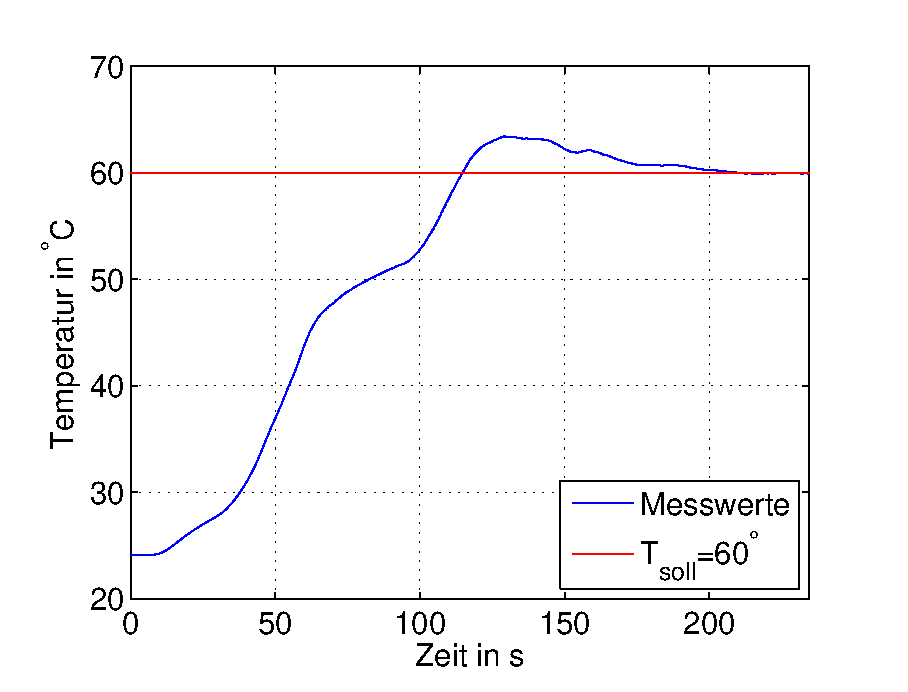
\includegraphics[scale=0.3]{./img/plots/2a.eps}
             \end{center}
             \end{figure}
    \end{columns}
\end{frame}
% subsection Manuelle REgelung: Kriterien für die Bestimmung der Stellgröße (end)
